\documentclass[11pt,a4paper,oneside]{report}
\usepackage[utf8]{inputenc}
\usepackage[english]{babel}
\usepackage{amsmath}
\usepackage{amsfonts}
\usepackage{amssymb}
\usepackage{graphicx}
\usepackage[left=2cm,right=2cm,top=2cm,bottom=2cm]{geometry}
\author{Daniel Aguiar da Silva Carvalho}
\begin{document}
\sffamily
\begin{center}
\textbf{\large{ALLOCATIONS DOCTORALES DE RECHERCHE ARC}}\\
\textbf{\large{Rapport d’activité 2016}}
\end{center}
\bigskip

\begin{flushleft}
\textbf{ARC No.:} 6\\
\bigskip

\textbf{Année d’obtention de l’ADR:} 2014\\
\bigskip

\textbf{Etablissement gestionnaire de la subvention (celui qui a établi le contrat de travail):} Université Jean Moulin Lyon 3\\
\bigskip

\textbf{Etablissement d’inscription en thèse:} Université Jean Moulin Lyon 3\\
\bigskip

\textbf{Titre du projet de thèse:} Trusted SLA-Guided Data Integration on Multi-Cloud Environment\\
\bigskip

\textbf{Nom \& prénom du bénéficiaire de l’ADR:} AGUIAR DA SILVA CARVALHO Daniel\\
\bigskip

\textbf{e-mail:} danielboni@gmail.com\\
\bigskip

\textbf{Nom du responsable de thèse:} GHEDIRA-GUEGAN Chirine\\
\bigskip

\textbf{e-mail:} chirine.ghedira-guegan@univ-lyon3.fr\\
\bigskip

\textbf{Intitulé et coordonnées complètes du laboratoire:} \\
Centre de Recherche Magellan (EA 3713, Lyon3) – Université Jean Moulin Lyon 3\\
6, Cours Albert Thomas\\
BP 8242\\
69355 Lyon cedex 08\\
Tél.: 04 78 78 71 58\\
centremagellan@univ-lyon3.fr\\
\bigskip

\textbf{Nom du Directeur:} Denis Travaille\\
\end{flushleft}

\newpage
\begin{flushleft}
\textbf{1. Objectifs et l’Originalité du sujet de thèse (2 pages maxi)}\\
\end{flushleft} 

Data integration is a widely studied issue in the database domain. It consists in merging data from different databases and providing a unified view of this data to the user~\cite{Lenzerini:2002}. Commonly, data integration is referred in the literature as a problem of answering queries using views. Many authors have reported their algorithms for this purpose~\cite{Halevy:2001}. Levy \textit{et al.} proposed the \textit{bucket algorithm}~\cite{Levy:1996}. It builds a \textit{bucket} for each subgoal in the query. A \textit{bucket} includes all views that can mapped to a given subgoal. Then, the algorithm generates combinations of the different buckets produced, and checks wheter each one is a rewriting of the query. Duschka and Genesereth introduced the \textit{inverse-rules algorithm}~\cite{Duschka:1997}. It produces a set of inverse rules (one for each subgoal in the view) from local views to the global view. Rewritings are obtained by unfolding the query in terms of the inverse rules produced. Pottinger and Halevy presented the \textit{MiniCon algorithm} in~\cite{Pottinger:2001}. It identifies a set of views that contains query subgoals. Once a views is selected, the algorithm creates mapping from the query subgoal to the view subgoal if the mapping of variables are possible. These mappings are named MiniCon description (MCD). Finally, a rewriting is a combination of MCDs covering all query subgoals and satisfying the relations between predicates. In general, algorithms in this domain share the same performance problem while combining views to produce a rewriting. Depending on the size of the query and the amount of available views, these algorithms requires a lot of computing resources and time to process the rewriting and integration. New architectures like the cloud open challenges to data integration.

Data integration can be seen in the cloud computing as a service composition problem. Selecting services and producing service compositions is computationally costly. Moreover, executing compositions can lead to retrieve and process data collections that can require an important amount of memory, storage and computing resources. Data integration solutions on the service-oriented domain deal with query rewriting problems. In our previous work~\cite{Carvalho2015}, we have identified trends and open issues regarding the use of SLA in data integration solutions on multi-cloud environments.
%
Barhamgi \textit{et al.} proposed a query rewriting approach which processes queries on data provider services~\cite{Barhamgi2010}. The query and data services are modeled as RDF views. A rewriting answer is a service composition in which the set of data service graphs fully satisfy the query graph.  
%
Benouaret \textit{et al.} introduced a service composition framework to answer preference queries~\cite{Benouaret2011}. In that approach, two algorithms based on~\cite{Barhamgi2010} are presented to rank the best rewritings based on previously computed scores.
%
Ba \textit{et al.} presented an algorithm based on \textit{MiniCon} that produces and order rewritings according to user preferences~\cite{ba2014}. The user preference concept is a score used to rank the order in which services are selected.
%
As in the database domain, these approaches requires an important amount of resources to process the rewriting and integration. 
%
It is important to review the existing data integration studies to be adapted to the cloud model. 

The cloud computing paradigm provides computing resources (as services) in an on-demand and scalable manner to cloud consumers. This on-demand provision and the pricing model imposed by the cloud changes the way data integration solutions should be tackled. Instead of designing processes and algorithms taking into account the limits on resources availability, the cloud sets focus on the economic cost allowing resource consumption and producing results while delivering data under subscription oriented cost models.

When a service is billed to a consumer, the provider and customer agree on price, quality guarantees and penalties associated to its violation in service level agreement (SLA) contracts. Several researches have reported their studies on SLA in different domains~\cite{AlhamadDC11}. In the cloud context, Rak \textit{et al.} proposed an approach to specify security requirement and to associate them to cloud services~\cite{rak2013}. Mavrogeorgi \textit{et al.} introduced a SLA management framework that allows the creation and enforcement of customized SLAs~\cite{Mavrogeorgi2013}. Leitner \textit{et al.} presented a approach to monitor and predict SLA violations before they impacted the provider's SLA~\cite{Leitner2010}. In general, proposals regarding SLAs in the deployment of services focus on two aspects: (\textit{i}) approaches focusing on the life cycle of the SLA mainly interested in the contract negotiation phase between the cloud and the service consumer; and (\textit{ii}) works monitoring contracts and cloud resources in order to avoid SLA violations, and consequently penalties due to its violation. In this sense, to the best of our knowledge, we have not identified any other approach that proposes the use of SLA associated to a data integration solution in a multi-cloud environment.

With growing needs and requirements, applications use different cloud providers for externalizing different data processing and management resources. This fact adds more challenges to data integration considering (i) the large amount and diversity of data; (ii) the user quality and security requirements of the integration; and (iii) the cloud heterogeneity in expressing and enforcing the corresponding clauses. Indeed, we believe that given the volume and the complexity of query evaluation, it is important to combine and revisit well-known data integration solutions and adapt them to this context. We strongly believe that this can be done according to quality of service requirements expressed by the consumers and service level agreement contracts exported by the cloud providers that host data collections and deliver resources for executing the associated management processes.

Considering the aforementioned, this thesis project intends to address data integration in a multi-cloud hybrid context. The originality of our approach consists in guiding the entire data integration solution taking into account (i) user preferences statements; (ii) SLA contracts exported by different cloud providers; and (iii) several QoS measures associated to data collections properties (for instance, trust, privacy, economic cost). The objective is to propose data integration strategies adapted to the vision of the economic model of the cloud such as (1) accepting partial results delivered on demand or under predefined subscription models that can affect the quality of the results; (2) accepting specific data duplication that can respect user preferences but ensure data availability; and (3) accepting to launch a task that contributes to an integration on a first cloud whose SLA verifies a given requirement rather than on a more powerful cloud but with less quality guarantees in the SLA.

In our work we consider an example from the domain of energy management. My directors are working on two national projects in this domain. So for instance, we assume we are interested in queries like: Give a list of energy providers that can provision 1000 KW-h, in the next 10 seconds, that are close to my city, with a cost of 0,50 Euro/KW-h and that are labeled as green? The question is how can the user efficiently obtain results for her queries such that they meet her QoS requirements, they respect her subscribed contracts with the involved cloud provider(s) and such that they do not neglect services contracts? Particularly, for queries that call several services deployed on different clouds. This work is part of an international collaboration with the DiMAp, Federal University of Rio Grande do Norte.

The project development is occurring naturally and well. In fact, this happens due to several aspects: (i) the close relationship and the easy access to my directors; (ii) the good frequency of meetings. Normally, we have at least one meeting for a week (that can be web conferences) in order to evaluate the status of the work; (iii) the research center infrastructure and team; and (iv) the monthly group meetings where we can discuss about the development of the projects with other colleagues. In addition, there are meetings in another laboratory, LIRIS. These moments are important because we can have an external view and comments about our research.

\newpage
\begin{flushleft}
\textbf{2. Synthèse du travail effectué dans l’année (2 pages maxi)}\\
\end{flushleft}

During the second year, we have been working on the development of our data integration approach. Given a query and a set of user preferences associated to it, the query execution process is divided in three phases. The figure 1 illustrates our data integration approach.

\begin{figure}[h!]
\center
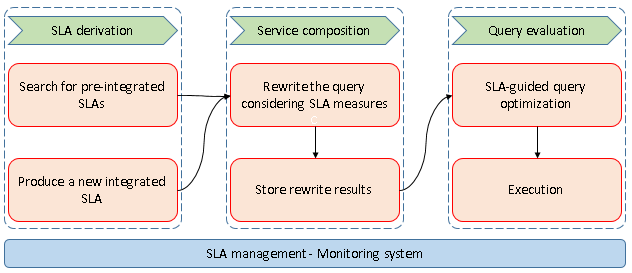
\includegraphics[scale=0.7]{../../general_approach.PNG} 
\caption{SLA-guided data integration approach}
\end{figure}

The first phase is the SLA derivation. It consists in looking for a (stored, integrated) SLA derived for a similar request. If a similar SLA is found, the request is forwarded to the query evaluation phase. Otherwise, a new integrated SLA is produced. The query is expressed as a service composition with associated user preferences (specified as SLA measures in the derived SLA). In the second phase, service composition, the query is rewritten in terms of different services considering the user preferences and the SLAs of each service involved in the composition. The rewriting result is stored for further uses. Finally, in the query evaluation phase, the query is optimized in terms of user preferences and SLAs concerning the consumed resources and the economic cost of the query. Once optimized, the query processed in the execution engine. In addition, we are assuming a SLA management module and monitoring system responsible to verify if the SLA contracts are being respected. We have worked on the phases two and three, firstly. 
%The following activities were developed to achieve our objectives:
	
\cite{ba2014} have proposed an algorithm for refining services composition. Their goal was to use user preferences to select and rank services in order to avoid the exponential problem while combining and producing compositions. Composition are incrementally produced until to reach a (predefined) desired number. In collaboration with our colleagues in Brazil (authors in~\cite{ba2014}), we have worked on an adapted version of \cite{ba2014} to our data integration solution. However, while performing the integrating we have identified some design issues that made it useless to our approach: (i) their concept of user preferences are scores associated to services previous defined by the user while, for us, user preferences are quality requirements expected by the user concerning the whole integration; (ii) their algorithm accepts rewriting including calls to services that are not interest for the composition. Assuming that on the cloud each service has a price associated to its request, this kind of composition can produced an extra value to the composition that is not interest and useful to the user. This adaptation process helped us to identify important issues to be applied to our own implementation.

%a) Adapting a previous query rewriting algorithm to our approach. This work was performed in collaboration with our colleagues in Brazil. The idea was to adapt a previous work from their lab to our data integration solution. While integrating we have identified some design problems that made it useless to our approach. However, the work in group help us to identify important issues to be applied to our own implementation.

%b) Query rewriting algorithms. We have produced a state of the art about query rewriting algorithm.  The approaches are divided into two different domains: database and service-oriented architecture. In the database domain, the different works concerning query rewriting using views have been studied in the literature. In general, the approaches deal with an exponential problem depending on the size of the query and the quantity of views. In the service-oriented domain, the approaches share the same problem. Producing services composition is extremely costly depending on the size of the composition (query) and the amount of services to be combined. Some approaches have tackled this issue. They have tried to minimize the effort to produce rewritings by considering user preferences or by limiting the desired number of rewritings. These works have been used as base and reference to produce our own algorithm.

Starting from the knowledge acquired while working on~\cite{ba2014}, we have produced a state of the art about query rewriting algorithm. The approaches can be divided into two domains: database and service-oriented architecture. In the database domain, studies (such as \cite{Duschka:1997,Levy:1996,Pottinger:2001}) have documented their approaches for answering queries using views. In general, while producing rewritings, these approaches suffer from the time exponential problem depending on the size of the query and the quantity of views. In the service-oriented domain, query rewriting can be seen as a service composition problem. Approaches (such as \cite{Barhamgi2010,Benouaret2011,Umberto}) share the same problem as on the database domain while producing services composition which is a task extremely costly depending on the size of the composition (query) and the amount of services to be combined. \cite{ba2014} have tried to minimize the effort to produce rewritings by considering user preferences (as scores) and by limiting the desired number of rewritings.

Based on the related work, we have developed and formalized the \textit{Rhone} service-based query rewriting algorithm guided by service level agreements (SLA). Our work address this issue and proposes the algorithm with two original aspects: (i) the user can express his quality preferences and associated them to his query; and (ii) service’s quality aspects defined in SLAs guide the service selection and the whole rewriting process.  Given a set of abstract services, a set of concrete services and a user query (both defined in terms of abstract services), and a set of user quality preferences, the \textit{Rhone} derives a set of service compositions that answer the query and that fulfill the quality preferences regarding the context of data service deployment. The algorithm consists in four steps: (i) \textit{Selecting concrete services}. Similar to~\cite{Levy:1996,Pottinger:2001} our algorithm selects services based on the abstract services that exists in the query, but it includes two differences: first, a concrete service cannot be select if it contains an abstract service that is not present in the query; and second, the service' quality aspects (extracted from its SLA) must be in accordance with the user quality preferences; (ii) \textit{creating mappings from concrete services to the query (called concrete service description (CSD))} inspired in~\cite{Pottinger:2001} including also the information concerning the services' SLA; (iii) \textit{combining CSDs}; and (iv) \textit{producing rewritings} until to fulfill the user requirements according to the services' SLA. Each phase of the algorithm and each concept (query, concrete services, mapping rules, for instance) were formally specified and described.

%d) Configuration of a multi-cloud environment. We have worked on the configuration of a multi-cloud environment. However, we found some problems at this point: (i) the configuration and deployment of cloud infrastructure using open source technologies is not easy and requires important technical skills while configuring the network resources; (ii) it requires a powerful machine. Due to that we have configured a simulation of cloud; and (iii) we have searched for private cloud providers, but they allow few access and power permissions to manage resources. In addition, they are quite expensive. We are still working on best way to manage this issue.

In order to evaluate our approach and the \textit{Rhone} algorithm, we have worked on configuration of a multi-cloud environment. We have searched for open source solutions instead of privates once they are (i) quite expensive; and (ii) do not allow to extend and access directly the different level of SLAs. The OpenStack was selected as our technology. We have installed and configured the different modules necessaries to the OpenStack. However, we have some issues: (i) the configuration and deployment of cloud infrastructure require important technical skills while configuring the network resources; (ii) it requires a powerful machine. Due to these reasons we have configured a simulation of cloud run our experiments.

The first version of the \textit{Rhone} was implemented using Java according to its formal definition. The algorithm was tested in a cloud simulation containing 35 services in its service registry. We have tested different types of query varying on the size and on the number of user preferences. Although our algorithm shares the same time performance problem as the previous approaches while combining compositions, the preliminary experiments have shown that the Rhone can enhance the quality in data integration by considering the user preferences and service’s quality aspects extracted from service level agreements. Our approach avoid selecting and using services to produce compositions that are not interest to the user once they do not fulfill his quality requirements. In addition, as result we have submitted short paper to EDBT 2016. 

We developed an improved version of the algorithm that manages better the manner in which lists of objects are managed. We have applied this version to a new set of experiments running 100 concrete services. With the results obtained from this experiment and the final version of our formalization, we are working on a new paper that included an extensive description of the algorithm and its evaluation to be submitted to ADBIS 2016 (deadline 27th March).

%h) SLA model to data integration. The state of the art on SLA have been analyzed to serve as basis to our SLA model. The works on SLA to cloud computing can be divided in two groups: (i) approaches dealing with the SLA negotiation phase. They focus on methods to stablish good and well-defined agreements between providers and customers; and (ii) works focus on monitoring/allocating resources in order to detect and avoid SLA violations. These works helped while proposing our SLA model and schema. Note that the SLA is the main concept in our proposal. It is responsible to guide the entire approach from the beginning to the end. There are some challenges regarding SLA: (i) once we are inserted into a multi-cloud context, we are dealing with a large heterogeneity of SLAs among different clouds. It is possible to have the same concept defined in a different way depending on the cloud; (ii) there are different levels of SLA: user SLAs, service SLAs and cloud SLAs. It is necessary to have a mapping between SLA measures that can be expressed in a different manner depending on the level; and (iii) it is possible to face a diversity chain of SLA from different levels and to map and identify measures is a hard process.

With this work performed, we have been developing our SLA model to data integration. As mentioned before, proposals to SLA in cloud computing can be divided in two groups: (i) approaches dealing with the SLA negotiation phase. They focus on methods to establish good and well-defined agreements between providers and customers; and (ii) works focus on monitoring/allocating resources in order to detect and avoid SLA violations. These works helped us while proposing our SLA model and schema. The SLA is the main concept in our proposal. It is responsible to guide the entire approach from the beginning to the end while fulfilling the user requirements. At this point, some challenges arises: (i) In a multi-cloud context, we are dealing with a large heterogeneity of SLAs among different clouds. Logically, an SLA measure can be defined in a different way depending on the cloud; (ii) there are different levels of SLA: user SLAs, service SLAs and cloud SLAs. Consequently, a user requirement defined in a user SLA is computed in terms of different measures on Service and Cloud SLAs. It is necessary to have a mechanism that maps and compute the user requirement and SLA measures; and (iii) it is possible to exists a chain of SLA, and to map and computed measures in this chain can require a hard processing. i) Paper to ADBIS and VLDB PhD consortium. Currently, we have been working on a paper that focus on the description of our SLA model, schema and data integration approach to be submitted to the VLDB PhD workshop (deadline 4 April).

%i) Paper to ADBIS and VLDB PhD consortium. Currently, with our last results, we have been working on two new papers: one concerning the algorithm to be submitted to ADBIS 2016 (deadline 27th March), and another one focusing on the SLA model, schema and data integration approach to be submitted to the VLDB PhD workshop (deadline 4 April).

\newpage
\begin{flushleft}
\textbf{3 Production scientifique}\\
\end{flushleft}

\noindent
D. A. S. Carvalho, N. Benani, C. Ghedira-Guegan, P. A. Souza Neto and G. Vargas-Solar. \textbf{A Query Rewriting Algorithm for Data Integration Quality (short paper)}. Submitted to 19th International Conference on Extending Database Technology (EDBT 2016).
\bigskip

\noindent
D. A. S. Carvalho, N. Benani, C. Ghedira-Guegan, P. A. Souza Neto and G. Vargas-Solar. \textbf{Rhone: a quality-based query rewriting algorithm for data integration}. To be submitted in 20th East-European Conference on Advances in Databases and Information Systems (ADBIS 2016).
\bigskip

\noindent
D. A. S. Carvalho, N. Benani, C. Ghedira-Guegan, P. A. Souza Neto and G. Vargas-Solar. \textbf{Quality-oriented data integration on multi-cloud environment}. To be submitted in VLDB PhD Workshop (collocated in the 42nd International Conference on Very Large Data Bases).
\bigskip

\noindent
\textbf{Poster presentation} in the « Journée Scientifique de l'Arc 6 » held in 20th November 2015 at Grenoble, France. 
\bigskip

\noindent
\textbf{PhD proposal and query rewriting algorithm presentation} to the Service-Oriented Computing team meeting from LIRIS, Lyon 1. In 3rd December 2015.
\bigskip

\noindent
\textbf{Query rewriting algorithm and ongoing works presentation} to the Information System group from the Magellan’s Research Center. In 4th February 2016.

\newpage
\begin{flushleft}
\textbf{4. Perspectives (1 page maxi)}\\
\end{flushleft}
Once we have been working on the phases two and three of our data integration approach, we are going to carry on completing what is missing on these phases. This concerns to build the module that threats the SLA model and extracts measures information to be used in the rewriting algorithm. With this work done, we are going to integrate both parts: the SLA module and the Rhone algorithm. 
The evaluation of the approach is essential and can be presented to partners in energy domain to validate the feasibility of our approach. Once the modules are connected, a set of experiments in a multi-cloud environment will be performed to evaluate our solution. The results analysis will be the basis to another scientific article. In parallel, we will carry on writing the thesis document. The table below describes our intended calendar. 

The following activities are:
\begin{enumerate}
\item Paper submission ADBIS: this paper aims to present the description and formalization of the Rhone service-based query rewriting algorithm, and the results of the experiments produced in a cloud simulation.
\item Paper submission VLDB PhD workshop: this paper describes our data integration approach focusing on the SLA model and schema.
\item Building the SLA Module. The idea is to implement the module responsible (i) to use the SLA model proposed and (ii) to extract information from a diversity of SLA and produce the inputs required to our rewriting algorithm.
\item Optimizing the Rhone algorithm. The goal is to minimize the loss in performance and show that our algorithm gain in time while avoiding to selecting and composing services that clearly violate the user preferences.
\item Integrating modules. The aim is to integrate the SLA module and the Rhone algorithm.
\item Producing and evaluating experiments. Once the different modules and the three phases of the approach are working integrated, experiments are going to be performed in a simulation of multi-cloud to evaluate the entire solution.
\item Producing a scientific paper. Naturally, the results obtained from the previous experiments is going to be used in another scientific production.
\item Writing the thesis.
\end{enumerate}

\begin{figure}[h!]
\center
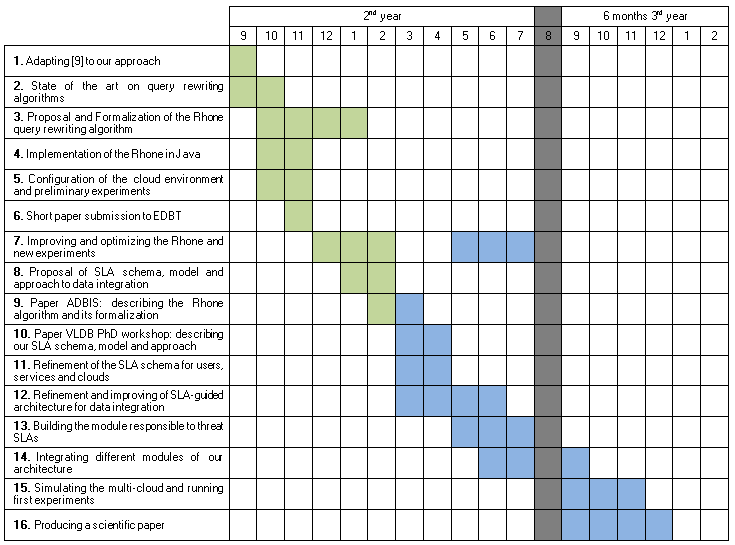
\includegraphics[scale=1]{calendar.png}
\end{figure}

\bibliographystyle{plain}
\bibliography{bibliography}


\end{document}